\documentclass[aspectratio=169]{beamer}
\usepackage{beamerthemesplit}
\usepackage{wrapfig}
\usetheme{SPbGU}
\usepackage{pdfpages}
\usepackage{array}
\usepackage{amsmath}
\usepackage{cmap} 
\usepackage[T2A]{fontenc} 
\usepackage[utf8]{inputenc}
\usepackage{indentfirst}
\usepackage{amsmath}
\usepackage{tikz}
\usepackage{multirow}
\usepackage[noend]{algpseudocode}
\usepackage{algorithm}
\usepackage{algorithmicx}
\usetikzlibrary{shapes,arrows}
\usepackage{fancyvrb}
\usepackage[english,russian]{babel}

\beamertemplatenavigationsymbolsempty


\title[Базы данных]{Базы данных}
\subtitle[]{}
% То, что в квадратных скобках, отображается в левом нижнем углу. 
\institute[СПбГУ]{
Программная инженерия \\
Санкт-Петербургский государственный университет
}

\author[Кутуев Владимир]{Кутуев Владимир}
\date{30 марта 2023г.}
\definecolor{orange}{RGB}{179,36,31}

\begin{document}
{
\begin{frame}
  
\includegraphics[width=1.7cm]{pictures/SPbGU_Logo.png}
  \vspace{-20pt}
  \begin{center}
    \titlepage
  \end{center}
\end{frame}
}

\begin{frame}[fragile]
  \transwipe[direction=90]
  \frametitle{А что вы знаете о базах данных?}
  
  \begin{center}
    
\includegraphics[height=.85\textheight]{pictures/Mem1.jpg}
  \end{center}
\end{frame}


\begin{frame}[fragile]
  \transwipe[direction=90]
  \frametitle{База данных}
  
  \begin{itemize}
    \item А collection of data stored according to a schema and manipulated according to the rules set out in one Data Modelling Facility \footnote{\href{https://www.iso.org/obp/ui/\#iso:std:iso-iec:tr:10032:ed-1:v1:en}{ISO/IEC TR 10032:2003}}
    \item An organized collection of data stored and accessed electronically \footnote{\href{https://en.wikipedia.org/wiki/Database}{Wikipedia}}
  \end{itemize}
\end{frame}

\begin{frame}[fragile]
  \transwipe[direction=90]
  \frametitle{СУБД}
  
  \begin{itemize}
    \item A collection of integrated services which support database management and together support and control the creation, use and maintenance of a database \footnote{\href{https://www.iso.org/obp/ui/\#iso:std:iso-iec:tr:10032:ed-1:v1:en}{ISO/IEC TR 10032:2003}}
    \item Software system that enables users to define, create, maintain and control access to the database \footnote{\href{https://en.wikipedia.org/wiki/Database\#Database_management_system}{Wikipedia}}
  \end{itemize}
\end{frame}

\begin{frame}[fragile]
  \transwipe[direction=90]
  \frametitle{Манипуляция данными}

  CRUD
  \begin{itemize}
    \item create
    \item read
    \item update
    \item delete
  \end{itemize}
\end{frame}

\begin{frame}[fragile]
  \transwipe[direction=90]
  \frametitle{ACID}

  \begin{itemize}
    \item atomicity --- Нельзя выполнить действие (транзакцию) не до конца
    \item consistency --- Транзакция переводит одно согласованное состояние в другое
    \item isolation --- Одно действие не может повлиять на другое (но есть нюанс)
    \item durability --- Сбои не должны повлиять на выполненные транзакции
  \end{itemize}
\end{frame}


\begin{frame}[fragile]
  \transwipe[direction=90]
  \frametitle{Архитектура ANSI-SPARC}
  
  \begin{tabular}{c c}
    \begin{minipage}{.6\textwidth}
      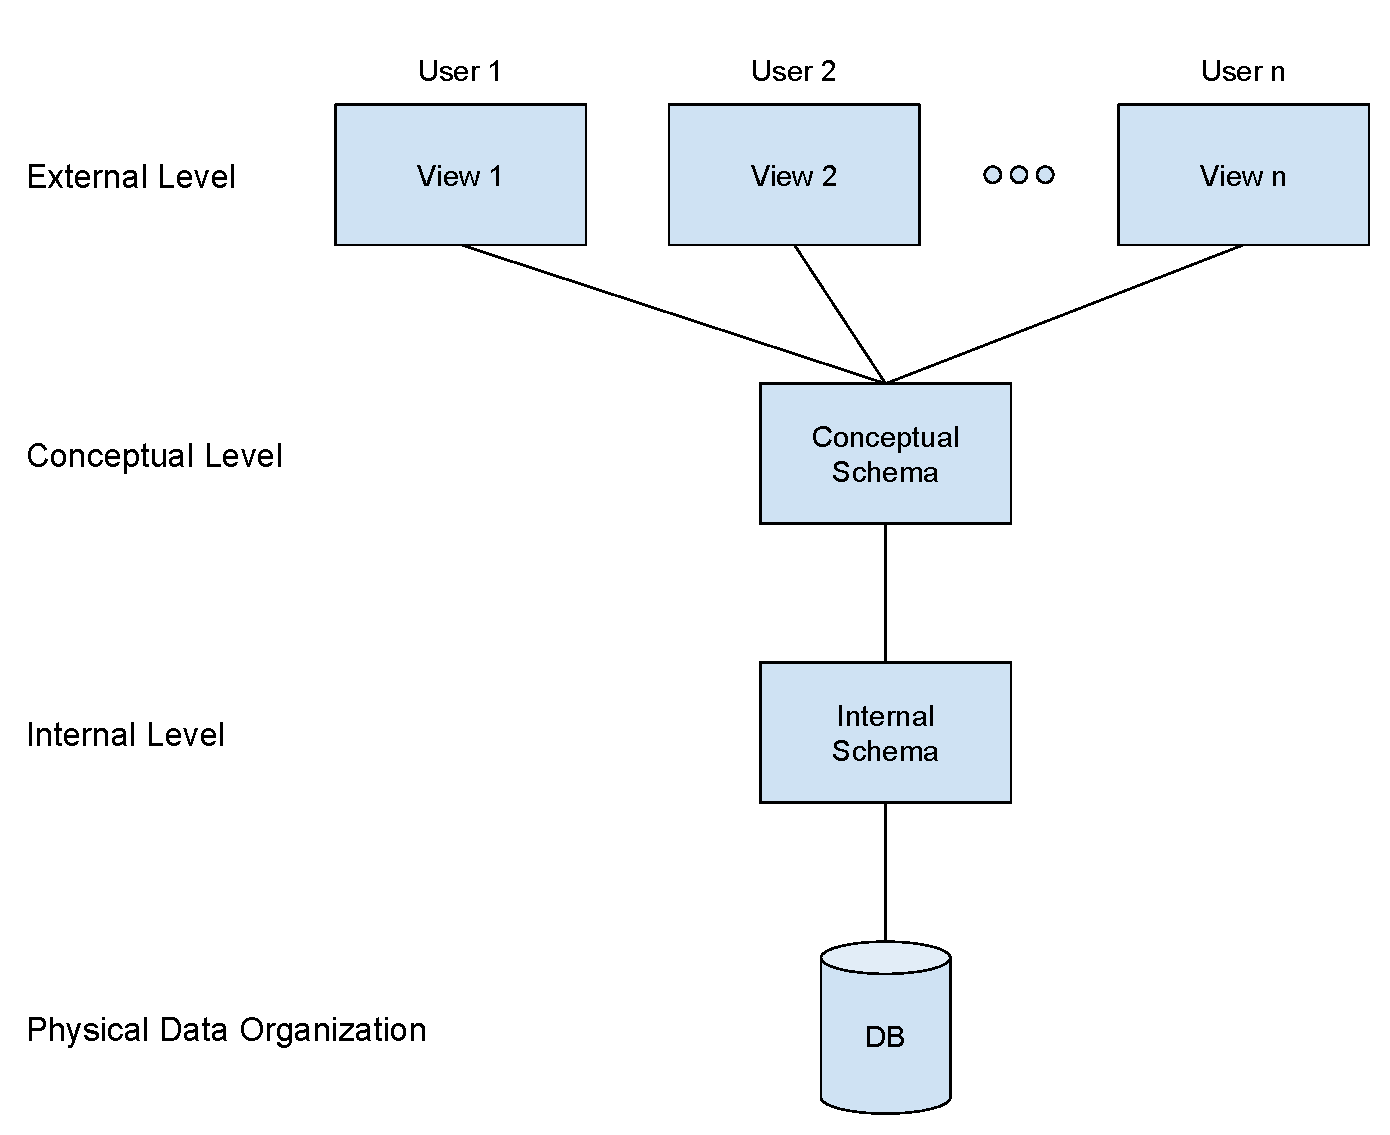
\includegraphics[width=\linewidth]{pictures/ANSI_SPARC.pdf} 
    \end{minipage}
    &
    \begin{minipage}{.35\textwidth}
    Модели данных
      \begin{itemize}
        \item Инфологическая --- представление данных с точки зрения пользователей
        \item Даталогическая --- представление данных с точки зрения администратора БД
        \item Физическая --- представление БД в памяти ПК
      \end{itemize}
    \end{minipage}
  \end{tabular}
\end{frame}

\begin{frame}[fragile]
  \transwipe[direction=90]
  \frametitle{Иерархическая модель}
  
  \begin{tabular}{c c}
    \begin{minipage}{.4\textwidth}
      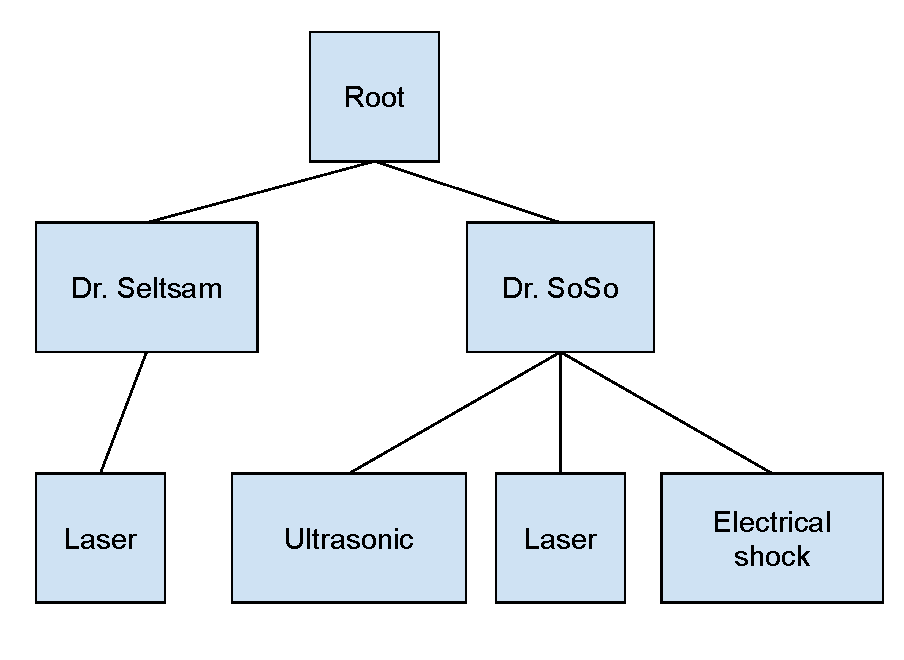
\includegraphics[width=\linewidth]{pictures/Hierarchical_model.pdf}
    \end{minipage}
    &
    \begin{minipage}{.55\textwidth}
      \begin{itemize}
        \item Данные --- записи с атрибутами, связанные с другими записями отношением 1:N
        \item Образуется древовидная структура
        \item Примеры СУБД
          \begin{itemize}
            \item IBM DBOMP --- конец 1960-х
            \item IBM IMS --- 1968
            \item InterSystems Caché --- 1997
          \end{itemize}
      \end{itemize}
    \end{minipage}
  \end{tabular}
\end{frame}

\begin{frame}[fragile]
  \transwipe[direction=90]
  \frametitle{Сетевая модель}
  
  \begin{tabular}{c c}
    \begin{minipage}{.4\textwidth}
      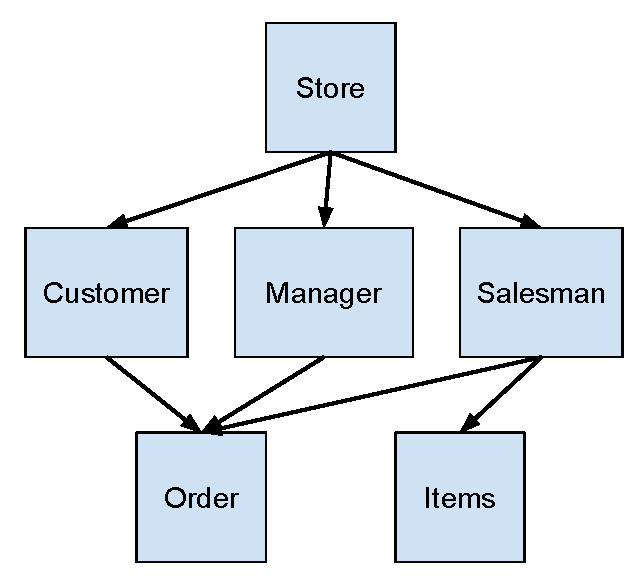
\includegraphics[width=\linewidth]{pictures/Network_model.pdf}
    \end{minipage}
    &
    \begin{minipage}{.55\textwidth}
      \begin{itemize}
        \item У одной записи может быть несколько предков и потомков --- граф общего вида (Циклы допустимы)
        \item Можно реализовывать связи 1:1, 1:N, M:N
        \item Примеры СУБД
          \begin{itemize}
            \item Integrated Data Store (IDS) --- 1960-е
            \item Integrated Database Management System (IDMS) --- 1973
          \end{itemize}
          \item Графовые СУБД
          \begin{itemize}
            \item Neo4j --- 2007
            \item TigerGraph DB --- 2017
            \item JanusGraph --- 2017
            \item ...
          \end{itemize}
      \end{itemize}
    \end{minipage}
  \end{tabular}
\end{frame}

\begin{frame}[fragile]
  \transwipe[direction=90]
  \frametitle{Реляционная модель}

  \begin{itemize}
    \item 1969-1970 годы Эдгар Кодд \footnote{\href{ https://www.seas.upenn.edu/~zives/03f/cis550/codd.pdf}{A Relational Model of Data for Large Shared Data Banks}}
    \item Можно реализовывать связи 1:1, 1:N, M:N
    \item Модель для большинства СУБД
    \item Примеры СУБД
      \begin{itemize}
        \item Oracle Database
        \item IBM DB2
        \item Microsoft SQL Server
        \item PostgreSQL
        \item MySQL
        \item SQLite
      \end{itemize}
  \end{itemize}
\end{frame}

\begin{frame}[fragile]
  \transwipe[direction=90]
  \frametitle{Реляционная модель}

  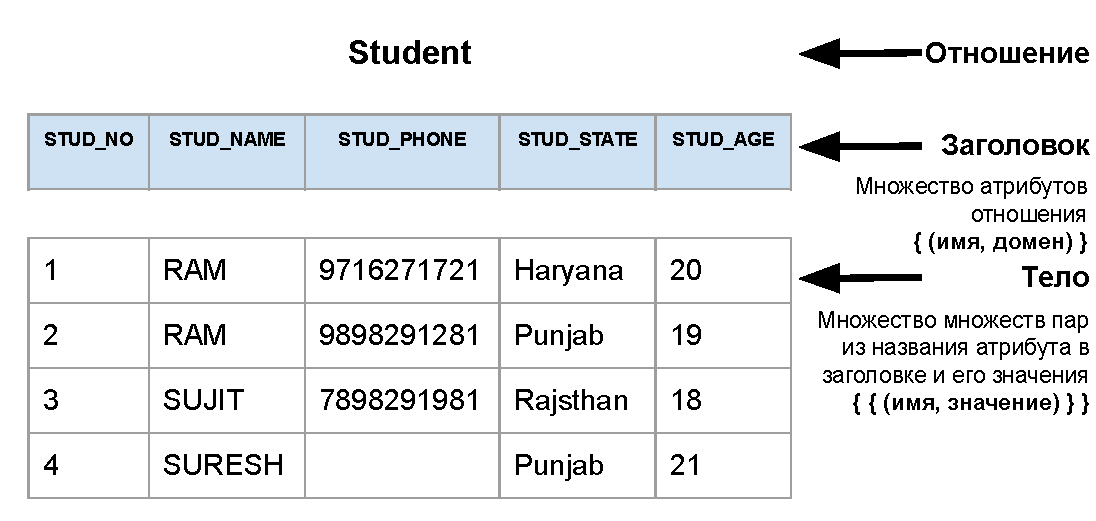
\includegraphics[width=\linewidth]{pictures/Relational_model.pdf}
\end{frame}

\begin{frame}[fragile]
  \transwipe[direction=90]
  \frametitle{Современные СУБД бывают}

  \begin{tabular}{cc}
    \begin{minipage}{.45\textwidth}
      Клиент-серверные
      \begin{itemize}
        \item Есть программа-сервер, которая монопольно взаимодействует с БД, приложения взаимодействуют с сервером
        \item Легче масштабировать
        \item Примеры
        \begin{itemize}
            \item MySQL
            \item PostgreSQL
            \item Neo4j
            \item ...
        \end{itemize}
      \end{itemize}
    \end{minipage}
    & 
    \begin{minipage}{.5\textwidth}
      Встраиваемые
      \begin{itemize}
        \item Нет отдельной программы-сервера, приложения взаимодействуют с БД непосредственно
        \item Высокая скорость и малый расход памяти (при небольших базах)
        \item Примеры
        \begin{itemize}
            \item SQLite
            \item Встраиваемые версии MySQL, Firebird, InterBase, Neo4j и др.
            \item ...
        \end{itemize}
      \end{itemize}
    \end{minipage}
  \end{tabular}
\end{frame}

\begin{frame}[fragile]
  \transwipe[direction=90]
  \frametitle{Способы взаимодействия с СУБД}

  \begin{tabular}{l l}
    <<Сырые>> запросы
    & 
    ORM/ODM/OGM (Object-\_ Mapping)
    \\
    \\
    \begin{minipage}{.45\textwidth}
      \begin{itemize}
        \item[+] Позволяют писать сложные запросы
        \item[+] Легче управлять оптимальностью запросов
        \item[--] Необходимо сопровождать в коде изменения схемы БД, или смену СУБД
        \item[--] Требуют аккуратности (инъекции!!!)
      \end{itemize}
    \end{minipage}
    & 
    \begin{minipage}{.5\textwidth}
      \begin{itemize}
        \item[+] Удобно для работы с небольшой схемой и несложными запросами
        \item[+] Автоматически генерируют скрипты миграции
        \item[+] Не надо учить ещё один язык
        \item[--] Требуют вычислительных ресурсов для своей работы
        \item[--] Невозможно/трудно выразить сложные запросы
      \end{itemize}
    \end{minipage}
  \end{tabular}
\end{frame}

\begin{frame}[fragile]
  \transwipe[direction=90]
  \frametitle{Практика}

  Инфологическая модель
  \begin{itemize}
    \item Пользователь
    \begin{itemize}
        \item Имя
        \item Номер телефона
    \end{itemize}
    \item Город
    \begin{itemize}
        \item Название
    \end{itemize}
    \item Пользователь живёт в каком-то городе, но может быть неизвестно, в каком городе он живёт
  \end{itemize}
  
\end{frame}

\begin{frame}[fragile]
  \transwipe[direction=90]
  \frametitle{Какой будет даталогическая модель?}
  
  \begin{center}
    
\includegraphics[height=.85\textheight]{pictures/Mem2.jpg}
  \end{center}
\end{frame}


\end{document}
